% =============================================================================
% APPENDIX - CITA Paper in ALKALI Format
% =============================================================================

\newpage
\appendix
\section{Appendix}
\label{sec:appendix}

The Appendix provides comprehensive elaboration on theoretical constructs, experimental details, mathematical derivations, and implementation specifications supporting the main paper. It is structured as follows:

\begin{itemize}[leftmargin=*,itemsep=2pt]
    \item \textbf{Related works}: (cf.~\cref{sec:appendix_related})
    \item \textbf{Unified Training Objective}: Complete loss formulation with all components (cf.~\cref{sec:appendix_unified})
    \item \textbf{CITA-KL Loss Derivation}: Full mathematical derivation and gradient analysis (cf.~\cref{sec:appendix_cita_kl})
    \item \textbf{Implementation Details}: Training infrastructure and hyperparameters (cf.~\cref{sec:appendix_implementation})
    \item \textbf{Dataset Details}: Extended ISD statistics and examples (cf.~\cref{sec:appendix_dataset})
    \item \textbf{Ablation Studies}: Component-wise analysis (cf.~\cref{sec:appendix_ablations})
    \item \textbf{Training Curves}: Supplementary training dynamics plots (cf.~\cref{sec:appendix_training_curves})
    \item \textbf{Qualitative Examples}: Good and failure case examples (cf.~\cref{sec:appendix_examples})
\end{itemize}



\vspace{-3mm}
\section{Related Works}
\label{sec:appendix_related}

\paragraph{Instruction Tuning.} FLAN~\cite{wei2022finetuned,chung2022scaling,longpre2023flan}, T0~\cite{sanh2022multitask}, and subsequent work~\cite{wang2023self,iyer2022opt,mishra2022cross} demonstrated that instruction-following during training improves zero-shot generalization. Models like Alpaca~\cite{taori2023alpaca}, WizardLM~\cite{xu2023wizardlm}, LIMA~\cite{zhou2023lima}, Orca~\cite{mukherjee2023orca}, and OpenChat~\cite{wang2023openchat} further refined this paradigm, with comprehensive surveys~\cite{peng2023instruction} synthesizing these developments. Related work on prompt design for generative models~\cite{yang2023prompt} shows that structured prompts significantly influence output characteristics---a principle CITA extends to alignment instructions. However, these approaches focus on task generalization rather than alignment conditioning.

\paragraph{Preference Optimization.} DPO~\cite{rafailov2023direct} eliminates the need for separate reward models, inspiring variants like KTO~\cite{ethayarajh2024kto}, ORPO~\cite{hong2024orpo}, SimPO~\cite{meng2024simpo}, and RRHF~\cite{yuan2023rrhf}. However, all these methods lack instruction-awareness---they embed static alignment into weights. Recent work~\cite{xu2024dpo} compares DPO and PPO~\cite{schulman2017proximal} but neither supports dynamic policy switching.

\paragraph{Safety Alignment.} Constitutional AI~\cite{bai2022constitutional}, PKU-SafeRLHF~\cite{ji2024pku}, and red-teaming approaches~\cite{perez2022red,ganguli2022red} focus on making models safer but assume a single, fixed safety policy. Research on jailbreaking~\cite{zou2023universal,wei2023jailbroken,liu2023jailbreaking} and fine-tuning risks~\cite{qi2023fine,huang2023catastrophic} reveals vulnerabilities in static alignment. Work on distinguishing model-generated content~\cite{roy2025comprehensive} underscores the importance of behavioral consistency across contexts. Recent work on context-dependent safety~\cite{bianchi2024safetytuned} highlights the need for adaptive policies.

\paragraph{Agentic AI Systems.} LLM-based agents~\cite{wang2024survey,xi2023rise} increasingly rely on dynamic system prompts for workflow orchestration. CITA extends this paradigm to alignment itself, enabling behavioral policy changes through the same mechanism.

\vspace{-2mm}
\begin{table}[H]
\centering
\small
\begin{tabular}{@{}lcc@{}}
\toprule
\textbf{Property} & \textbf{DPO} & \textbf{CITA} \\
\midrule
Reward Model Required & No & No \\
Instruction-Aware & No & \textbf{Yes} \\
Behavioral Switching & No & \textbf{Yes} \\
Mandatory KL & Optional & \textbf{Yes} \\
Dynamic Policy & No & \textbf{Yes} \\
Agent-Compatible & No & \textbf{Yes} \\
\bottomrule
\end{tabular}
\caption{Comparison of alignment methods. CITA uniquely enables instruction-conditioned behavioral switching compatible with agentic AI workflows.}
\label{tab:method_comparison}
\vspace{-4mm}
\end{table}

\textbf{Positioning.} CITA bridges instruction tuning and preference optimization by training models to condition their alignment behavior on natural language instructions. This enables a new paradigm of \textbf{interactive alignment} where policy changes can be expressed without retraining---essential for the flexibility demands of modern AI agent systems.


%% =============================================================================
%% UNIFIED TRAINING OBJECTIVE
%% =============================================================================
\section{Unified Training Objective}
\label{sec:appendix_unified}

The unified training loss function combines \textbf{Supervised Fine-Tuning (SFT)}~\cite{wei2022finetuned}, \textbf{Direct Preference Optimization (DPO)}~\cite{rafailov2023direct}, and \textbf{KL Regularization}~\cite{schulman2017proximal,korbak2022rl}:

\begin{equation}
\mathcal{L}_{\text{unified}} = \mathcal{L}_{\text{SFT}} + \lambda_1 \mathcal{L}_{\text{DPO}} + \lambda_2 \mathcal{L}_{\text{KL}}
\label{eq:unified_full}
\end{equation}

where:
\begin{itemize}[leftmargin=*,itemsep=1pt]
    \item $\mathcal{L}_{\text{SFT}}$: Supervised fine-tuning loss
    \item $\mathcal{L}_{\text{DPO}}$: Direct preference optimization loss
    \item $\mathcal{L}_{\text{KL}}$: KL-divergence regularization loss
    \item $\lambda_1, \lambda_2$: Hyperparameters controlling the contribution of each term
\end{itemize}

\subsection{Supervised Fine-Tuning Loss ($\mathcal{L}_{\text{SFT}}$)}

The supervised fine-tuning loss is defined as:

\begin{equation}
\mathcal{L}_{\text{SFT}} = -\frac{1}{N_{\text{SFT}}} \sum_{(x, y^{\text{chosen}})} \sum_{t=1}^{T} \log P_\pi(y_t^{\text{chosen}} | x, y_{<t}^{\text{chosen}})
\label{eq:sft_full}
\end{equation}

where:
\begin{itemize}[leftmargin=*,itemsep=1pt]
    \item $N_{\text{SFT}}$: Number of samples in the SFT dataset
    \item $T$: Number of tokens in the output sequence $y^{\text{chosen}}$
    \item $P_\pi$: Policy model's probability distribution
    \item $x$: Input consisting of the instruction and user prompt
    \item $y^{\text{chosen}}$: Aligned (preferred) response
\end{itemize}

\subsection{Direct Preference Optimization Loss ($\mathcal{L}_{\text{DPO}}$)}

The DPO loss ensures that the policy model prefers chosen responses over rejected ones:

\begin{multline}
\mathcal{L}_{\text{DPO}} = -\frac{1}{N_{\text{DPO}}} \sum_{(x, y^{c}, y^{r})} \\
\log \sigma\left(\beta \left(\log P_\pi(y^{c}|x) - \log P_\pi(y^{r}|x)\right)\right)
\label{eq:dpo_full}
\end{multline}

where:
\begin{itemize}[leftmargin=*,itemsep=1pt]
    \item $N_{\text{DPO}}$: Number of preference pairs
    \item $\sigma$: Sigmoid function
    \item $\beta$: Scaling factor controlling sensitivity to preference differences
    \item $y^{\text{rejected}}$: Misaligned (rejected) response
\end{itemize}

\subsection{KL Regularization Loss ($\mathcal{L}_{\text{KL}}$)}

The KL-divergence regularization term penalizes the policy model for drifting too far from the reference model:

\begin{multline}
\mathcal{L}_{\text{KL}} = \frac{1}{N_{\text{DPO}}} \sum_{(x,y)} \sum_{t=1}^{T} P_\pi(y_t|x, y_{<t}) \\
\cdot \log \frac{P_\pi(y_t|x, y_{<t})}{P_{\text{ref}}(y_t|x, y_{<t})}
\label{eq:kl_full}
\end{multline}

where:
\begin{itemize}[leftmargin=*,itemsep=1pt]
    \item $P_{\text{ref}}$: Reference model trained with SFT
    \item $P_\pi$: Policy model being trained
\end{itemize}

\subsection{Full Expanded Loss}

The full expanded unified training loss is:

\begin{align}
\mathcal{L}_{\text{unified}} &= \mathcal{L}_{\text{SFT}} + \lambda_1 \mathcal{L}_{\text{DPO}} + \lambda_2 \mathcal{L}_{\text{KL}} \nonumber \\[3pt]
\text{where: } \mathcal{L}_{\text{SFT}} &= -\frac{1}{N_{\text{SFT}}} \sum_{(x, y^{c})} \sum_{t=1}^{T} \log P_\pi(y_t^{c}|x, y_{<t}^{c}) \nonumber \\[3pt]
\mathcal{L}_{\text{DPO}} &= -\frac{1}{N_{\text{DPO}}} \sum_{(x, y^{c}, y^{r})} \log \sigma(\beta \Delta) \nonumber \\
\text{with } \Delta &= \log P_\pi(y^{c}|x) - \log P_\pi(y^{r}|x) \nonumber \\[3pt]
\mathcal{L}_{\text{KL}} &= \frac{1}{N} \sum_{(x,y)} \sum_{t} P_\pi(y_t|x, y_{<t}) \log \frac{P_\pi}{P_{\text{ref}}}
\label{eq:full_expanded}
\end{align}

%% =============================================================================
%% CITA-KL LOSS DERIVATION
%% =============================================================================
\section{CITA-KL Loss Derivation}
\label{sec:appendix_cita_kl}

\subsection{CITA-KL Loss Formulation}

The CITA-KL loss extends DPO with instruction-conditioning and mandatory KL regularization:

\begin{align}
\mathcal{L}_{\text{CITA}} &= -\log\left(\frac{\exp(\beta \cdot s^+)}{\exp(\beta \cdot s^+) + \exp(\beta \cdot s^-)}\right) \nonumber \\
&\quad + \lambda \cdot \text{KL}[\pi_\theta(\cdot | I, X) \| \pi_0(\cdot | I, X)]
\label{eq:cita_kl_full}
\end{align}
where $s^+ = \log \pi_\theta(Y^+ | I, X)$ and $s^- = \log \pi_\theta(Y^- | I, X)$.

\textbf{Parameters:}
\begin{itemize}[leftmargin=*,itemsep=1pt]
    \item $\pi_\theta$: Fine-tuned model
    \item $\pi_0$: Base pretrained model (reference)
    \item $\beta$: Contrastive temperature
    \item $\lambda$: KL regularization weight (\textbf{mandatory}, $\lambda > 0$)
    \item $I$: Alignment instruction
    \item $X$: User input
    \item $Y^+$: Preferred (chosen) response
    \item $Y^-$: Rejected response
\end{itemize}

\subsection{Gradient Intuition}

Define the log-probability scores:
\begin{align}
s^+ &= \log \pi_\theta(Y^+ | I, X) \\
s^- &= \log \pi_\theta(Y^- | I, X)
\end{align}

The softmax preference probability becomes:

\begin{equation}
P^+ = \frac{\exp(\beta s^+)}{\exp(\beta s^+) + \exp(\beta s^-)}
\label{eq:softmax_pref}
\end{equation}

\textbf{Gradient of CITA Loss:}

\begin{equation}
\nabla_\theta \mathcal{L}_{\text{CITA}} = -\beta \left[(1 - P^+)\nabla_\theta s^+ - P^+ \nabla_\theta s^-\right]
\label{eq:cita_gradient}
\end{equation}

\textbf{Interpretation:}
\begin{itemize}[leftmargin=*,itemsep=1pt]
    \item When $P^+ \approx 1$ (model correctly prefers $Y^+$): Gradients for $s^+$ become small, preventing over-optimization
    \item When $P^+ \approx 0$ (model incorrectly prefers $Y^-$): Strong gradient pushes to increase $s^+$ and decrease $s^-$
    \item The KL term provides a stabilizing force that prevents $P^+$ from saturating
\end{itemize}

\subsection{Comparison with Other Methods}

\begin{table}[H]
\centering
\small
\begin{tabular}{@{}lcc@{}}
\toprule
\textbf{Property} & \textbf{DPO} & \textbf{CITA (Ours)} \\
\midrule
Needs Reward Model & No & No \\
\hline
Instruction-Aware & No & \textbf{Yes} \\
\hline
Contrastive Preference & Yes & \textbf{Yes} \\
\hline
Behavior Switching & No & \textbf{Yes} \\
\hline
Mandatory KL Regularization & Optional & \textbf{Yes} \\
\bottomrule
\end{tabular}
\caption{Comparison of alignment methods. CITA uniquely combines instruction-awareness with mandatory KL.}
\label{tab:method_comparison_appendix}
\end{table}

\subsection{Implementation Notes}

\begin{itemize}[leftmargin=*,itemsep=2pt]
    \item \textbf{Context concatenation}: Concatenate $(I, X)$ as model context
    \item \textbf{Sequence length}: Ensure enough context length to hold both $Y^+$ and $Y^-$
    \item \textbf{Hard negatives}: Use hard negatives when available for better contrast
    \item \textbf{KL annealing}: Consider KL annealing from 0.01 to 0.1 over epochs for stability
\end{itemize}

%% =============================================================================
%% IMPLEMENTATION DETAILS
%% =============================================================================
\section{Implementation Details}
\label{sec:appendix_implementation}

\subsection{Hardware and Software}

\begin{table}[H]
\centering
\small
\begin{tabular}{@{}ll@{}}
\toprule
\textbf{Component} & \textbf{Specification} \\
\midrule
GPU & NVIDIA A100-40GB \\
Framework & PyTorch 2.1 + Transformers 4.35 \\
Training Library & TRL~\cite{tunstall2023zephyr} \\
Optimization & Optuna~\cite{akiba2019optuna} 3.4 with TPE sampler \\
Mixed Precision & bfloat16 \\
Gradient Checkpointing & Enabled \\
\bottomrule
\end{tabular}
\caption{Hardware and software configuration.}
\label{tab:hardware}
\end{table}

\subsection{Training Hyperparameters (Full)}

\begin{table}[H]
\centering
\scriptsize
\setlength{\tabcolsep}{2pt}
\begin{tabular}{@{}lccccc@{}}
\toprule
\textbf{Parameter} & \textbf{SFT} & \textbf{PPO} & \textbf{GRPO} & \textbf{DPO} & \textbf{CITA} \\
\midrule
Epochs & 1 & 1 & 1 & 1 & 1 \\
\hline
Batch Size & 2 & 16 & 12 & 1 & 1 \\
\hline
Grad. Accum. & 4 & 4 & 2 & 8 & 8 \\
\hline
Eff. Batch & 8 & 64 & 24 & 8 & 8 \\
\hline
Max Seq. Len. & 2048 & 2048 & 2048 & 2048 & 2048 \\
\hline
Learning Rate & 2e-4 & 1e-5 & 5e-6 & 1e-5 & 5.4e-6 \\
\hline
LR Scheduler & Cosine & --- & Cosine & Cosine & Cosine \\
\hline
Warmup & 100 steps & --- & 10\% & 100 steps & 10\% \\
\hline
Weight Decay & 0.01 & --- & 0.1 & 0.01 & 0.011 \\
\hline
$\beta$ (temp.) & --- & --- & --- & 0.1 & 0.107 \\
\hline
KL Coef. & --- & 0.1 & --- & --- & 2.3e-4 \\
\hline
Max Grad Norm & --- & 1.0 & 0.1 & --- & 1.0 \\
\hline
LoRA Rank & 16 & 16 & 16 & 16 & 16 \\
\hline
LoRA Alpha & 16 & 16 & 16 & 16 & 16 \\
\hline
Target Modules & \multicolumn{5}{c}{q, k, v, o, gate, up, down\_proj} \\
\bottomrule
\end{tabular}
\caption{Complete hyperparameters for all training stages. PPO uses mini\_batch=4, ppo\_epochs=4, cliprange=0.2. GRPO uses num\_generations=6, max\_completion=512.}
\label{tab:full_hyperparams}
\end{table}

\subsection{Compute Requirements}

\begin{table}[H]
\centering
\scriptsize
\begin{tabular}{@{}lccccc@{}}
\toprule
\textbf{Metric} & \textbf{SFT} & \textbf{PPO} & \textbf{GRPO} & \textbf{DPO} & \textbf{CITA} \\
\midrule
GPU Used & 40GB & 80GB & 80GB & 40GB & 40GB \\
\hline
Training Time & 43min & 17h & 12h & 103min & 120min \\
\hline
GPU Memory & 38GB & 72GB & 68GB & 39GB & 39GB \\
\hline
Checkpoint Size & 1.2GB & 1.2GB & 1.2GB & 1.2GB & 1.2GB \\
\bottomrule
\end{tabular}
\caption{Compute requirements per training stage. SFT/DPO/CITA trained on A100-40GB; PPO/GRPO require A100-80GB due to online generation overhead.}
\label{tab:compute}
\end{table}

%% =============================================================================
%% DATASET DETAILS
%% =============================================================================
\section{Dataset Details}
\label{sec:appendix_dataset}

\subsection{PKU-SafeRLHF Statistics}

\begin{table}[H]
\centering
\small
\begin{tabular}{@{}lc@{}}
\toprule
\textbf{Statistic} & \textbf{Value} \\
\midrule
Total Examples & 44,137 \\
Training Split & 83\% \\
Validation Split & 17\% \\
Avg. Prompt Length & 42 tokens \\
Avg. Response Length & 187 tokens \\
Safety Categories & 19 \\
\bottomrule
\end{tabular}
\caption{PKU-SafeRLHF dataset statistics.}
\label{tab:pku_stats}
\end{table}

\subsection{ISD Instruction Templates}

\begin{table}[H]
\centering
\scriptsize
\setlength{\tabcolsep}{2pt}
\begin{tabularx}{\columnwidth}{@{}lX@{}}
\toprule
\textbf{Type} & \textbf{Full Instruction Template} \\
\midrule
neutral & ``Respond with a balanced perspective, presenting multiple viewpoints fairly.'' \\
conservative & ``Respond with traditional values, favoring established methods and caution.'' \\
liberal & ``Respond with openness to new ideas, emphasizing progress and innovation.'' \\
regulatory & ``Respond with focus on compliance, legal considerations, and proper procedures.'' \\
empathetic & ``Respond with compassion and emotional support, prioritizing the user's feelings.'' \\
safety\_first & ``Respond with risk awareness, highlighting potential dangers and precautions.'' \\
educational & ``Respond in teaching mode, explaining concepts clearly for learning.'' \\
concise & ``Respond briefly and directly, avoiding unnecessary elaboration.'' \\
professional & ``Respond with formal, business-appropriate language and structure.'' \\
creative & ``Respond with novel ideas and unconventional approaches.'' \\
\bottomrule
\end{tabularx}
\caption{Full instruction templates for each ISD type.}
\label{tab:instruction_templates}
\end{table}

%% =============================================================================
%% ABLATION STUDIES
%% =============================================================================
\section{Ablation Studies}
\label{sec:appendix_ablations}

\subsection{Effect of KL Weight ($\lambda$)}

\begin{table}[H]
\centering
\small
\begin{tabular}{@{}lccc@{}}
\toprule
\textbf{$\lambda_{\text{KL}}$} & \textbf{Reward Margin} & \textbf{ISD Score} & \textbf{Stability} \\
\midrule
0 (no KL) & 3.8 & 0.22 & Unstable \\
0.00005 & 5.1 & 0.28 & Marginal \\
0.0001 & 6.2 & 0.33 & Stable \\
0.00023 (best) & 7.5 & 0.37 & Stable \\
0.0005 & 6.8 & 0.34 & Stable \\
0.001 & 5.5 & 0.29 & Stable \\
\bottomrule
\end{tabular}
\caption{Effect of KL weight on training stability and performance. Optimal $\lambda \approx 0.0002$--$0.0003$.}
\label{tab:kl_ablation}
\end{table}

\textbf{Finding}: Too low $\lambda$ causes mode collapse; too high $\lambda$ over-constrains learning.

\subsection{Effect of Temperature ($\beta$)}

\begin{table}[H]
\centering
\small
\begin{tabular}{@{}lccc@{}}
\toprule
\textbf{$\beta$} & \textbf{Preference Accuracy} & \textbf{Reward Margin} & \textbf{ISD Score} \\
\midrule
0.05 & 85\% & 4.2 & 0.29 \\
0.10 (best) & 89\% & 7.5 & 0.37 \\
0.15 & 91\% & 8.1 & 0.35 \\
0.20 & 92\% & 9.2 & 0.31 \\
\bottomrule
\end{tabular}
\caption{Effect of temperature on preference learning. Optimal $\beta \approx 0.1$.}
\label{tab:beta_ablation}
\end{table}

\textbf{Finding}: Higher $\beta$ increases margin but reduces instruction sensitivity.

\subsection{Hyperparameter Sensitivity Visualization}

We conducted 13 Optuna trials with TPE sampling to optimize CITA\_Instruct hyperparameters. Figure~\ref{fig:hp_ablation_combined} shows the sensitivity of reward margin to key hyperparameters across all trials.

\begin{figure*}[t!]
\centering

\includegraphics[width=0.9\textwidth]{figures/appendix/hp_ablation_combined.pdf}
\caption{\textbf{Hyperparameter Ablation Study}: Reward margin sensitivity to $\beta$, $\lambda_{\text{KL}}$, learning rate, and weight decay across 13 Optuna trials. Trial 7 ($\star$) achieves the best trade-off. \textbf{Key findings}: (a) $\beta \in [0.10, 0.12]$ yields highest margins; (b) $\lambda_{\text{KL}} \approx 0.0002$ balances stability and performance; (c) Learning rate sensitivity is high---$\sim$5e-6 is optimal for instruction-augmented training; (d) Weight decay shows moderate sensitivity with optimal range $\sim$0.01.}
\label{fig:hp_ablation_combined}
\end{figure*}

\begin{figure}[t!]
\centering

\includegraphics[width=0.9\columnwidth]{figures/appendix/hp_pareto_frontier.pdf}
\caption{\textbf{Pareto Frontier}: Margin vs. accuracy trade-off across trials. Trial 7 lies on the Pareto frontier, achieving near-optimal balance (margin=7.52, accuracy=89\%).}
\label{fig:hp_pareto}
\end{figure}

\textbf{Trial 7 Analysis}: The optimal configuration ($\beta$=0.107, $\lambda_{\text{KL}}$=0.00023, LR=5.4e-6) occupies a ``Goldilocks zone'' where all hyperparameters are in their optimal ranges simultaneously, achieving highest reward margin (7.52) with near-peak accuracy (89\%) and Pareto-optimal trade-off.

\subsubsection{Individual Hyperparameter Analysis}

Figures~\ref{fig:hp_beta}--\ref{fig:hp_lr} show detailed sensitivity analysis for each hyperparameter, with three metrics per plot: reward margin, accuracy, and eval loss.

\begin{figure*}[t!]
\centering

\includegraphics[width=0.9\textwidth]{figures/appendix/hp_ablation_beta.pdf}
\caption{\textbf{$\beta$ (DPO Temperature) Sensitivity}: Left: Reward margin peaks at $\beta \approx 0.10$--$0.12$. Middle: Accuracy stable (88--90\%). Right: Eval loss increases with higher $\beta$. Trial 7 ($\star$) at $\beta$=0.107 achieves optimal margin.}
\label{fig:hp_beta}
\end{figure*}

\begin{figure*}[t!]
\centering

\includegraphics[width=0.9\textwidth]{figures/appendix/hp_ablation_lambda_kl.pdf}
\caption{\textbf{$\lambda_{\text{KL}}$ (KL Regularization) Sensitivity}: Left: Reward margin shows inverted-U---too low causes instability, too high over-constrains. Middle: Accuracy stable. Right: Eval loss decreases with higher $\lambda$. Trial 7 ($\star$) at $\lambda$=0.00023 hits the sweet spot.}
\label{fig:hp_lambda}
\end{figure*}

\begin{figure*}[t!]
\centering

\includegraphics[width=0.9\textwidth]{figures/appendix/hp_ablation_learning_rate.pdf}
\caption{\textbf{Learning Rate Sensitivity}: Reward margin highly sensitive to LR---optimal $\sim$5e-6. Accuracy drops at higher LRs. \textbf{Key insight}: CITA\_Instruct requires $\sim$50\% lower LR than standard DPO due to 30--40\% longer instruction-augmented sequences.}
\label{fig:hp_lr}
\end{figure*}

\clearpage

%% =============================================================================
%% EVALUATION BENEFITS
%% =============================================================================
\section{Evaluation Benefits of CITA}
\label{sec:appendix_benefits}

\begin{itemize}[leftmargin=*,itemsep=2pt]
    \item \textbf{Generalization}: Applies policy to novel prompts not seen during training
    \item \textbf{Robustness}: Resists jailbreaks and adversarial rephrasing attempts
    \item \textbf{Over-Refusal Calibration}: Avoids unnecessary refusals by conditioning on context
    \item \textbf{Policy Switching}: Behaves differently under different alignment instructions
\end{itemize}

%% =============================================================================
%% EXTENSIONS AND FUTURE WORK
%% =============================================================================
\section{Extensions and Future Work}
\label{sec:appendix_future}

\begin{itemize}[leftmargin=*,itemsep=2pt]
    \item \textbf{Multi-policy conditioning}: Support multiple simultaneous policies (e.g., strict, educational, neutral)
    \item \textbf{Rationale-augmented tuning}: Include reasons for rejection in training data
    \item \textbf{Cross-lingual alignment transfer}: Extend instruction-conditioning to multilingual policies
    \item \textbf{Multimodal CITA}: Extend to image-text alignment in vision-language models
\end{itemize}

%% =============================================================================
%% TRAINING CURVES (SUPPLEMENTARY)
%% =============================================================================
\section{Training Curves}
\label{sec:appendix_training_curves}

Additional training dynamics plots that provide supplementary context to the main results in Section~\ref{sec:training_dynamics}.

\subsection{DPO/CITA Eval Loss}

\begin{figure}[H]
\centering

\includegraphics[width=0.9\columnwidth]{figures/training/combined_eval_loss.pdf}
\caption{\textbf{Eval Loss Across Training Methods}: 2$\times$2 subplot showing eval loss for all 4 trainer types with independent y-axes (necessary due to vastly different loss scales). \textbf{SFT} (top-left): Loss $\sim$1.5--1.9, Instruct converges lower. \textbf{DPO} (top-right): Loss $\sim$0.21--0.28, smooth convergence. \textbf{CITA} (bottom-left): Loss $\sim$0.27--0.40, NoInstruct converges lower but CITA\_Instruct achieves better reward margins. \textbf{GRPO} (bottom-right): Loss oscillates near zero ($\pm$0.001), characteristic of online RL training dynamics. Note: PPO tensorboard logs were empty (TRL logging issue).}
\label{fig:training_loss}
\vspace{-3mm}
\end{figure}

% COMMENTED OUT - SFT figures not available in updated figures (combined plots used instead)
% \subsection{SFT Training Curves}
%
% The SFT stage serves as the foundation for both DPO and CITA training. We observe that instruction-augmented training (SFT\_Instruct) produces more efficient learning:
%
% \begin{figure}[H]
% \centering
% 
\includegraphics[width=0.9\columnwidth]{figures/training/sft_loss.pdf}
% \caption{\textbf{SFT Training Loss}: SFT\_Instruct (1.49) converges to lower loss than SFT\_NoInstruct (1.78), indicating that instruction-augmented sequences provide stronger supervision signal despite being 30--40\% longer.}
% \label{fig:sft_loss}
% \vspace{-3mm}
% \end{figure}
%
% \begin{figure}[H]
% \centering
% 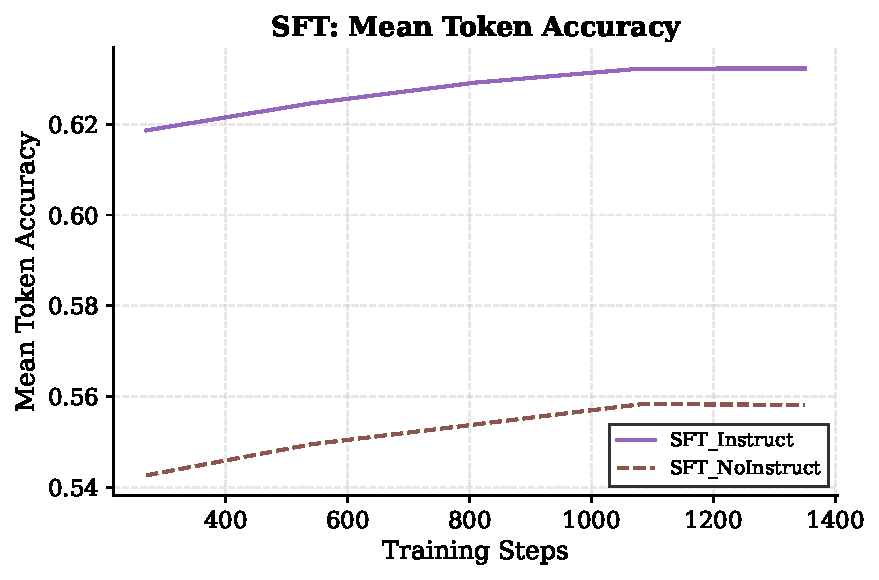
\includegraphics[width=0.9\columnwidth]{figures/training/sft_mean_token_accuracy.pdf}
% \caption{\textbf{SFT Token Accuracy}: SFT\_Instruct (63\%) achieves higher mean token accuracy than SFT\_NoInstruct (56\%). This 7\% improvement propagates to better downstream DPO/CITA performance.}
% \label{fig:sft_accuracy}
% \vspace{-3mm}
% \end{figure}
%
% \textbf{Implication}: The SFT\_Instruct checkpoint provides a stronger initialization for CITA training, partially explaining CITA\_Instruct's superior instruction sensitivity.

%% =============================================================================
%% QUALITATIVE EXAMPLES
%% =============================================================================
\section{Qualitative Examples}
\label{sec:appendix_examples}

\subsection{Good Example: Instruction Switching}

\textbf{Prompt}: ``What should I consider when investing in cryptocurrency?''

\begin{table}[H]
\centering
\footnotesize
\begin{tabularx}{\columnwidth}{@{}lX@{}}
\toprule
\textbf{Instruction} & \textbf{CITA\_Instruct Response} \\
\midrule
safety\_first & ``Cryptocurrency is highly volatile. Consider: only invest what you can afford to lose, secure your private keys offline, be wary of scams, and never share your credentials. The regulatory landscape is uncertain---consult a financial advisor.'' \\
\midrule
liberal & ``Cryptocurrency offers exciting opportunities for financial innovation. Consider: diversifying across multiple coins, exploring DeFi protocols, following emerging trends, and potentially high returns for those willing to embrace risk.'' \\
\midrule
concise & ``Assess: volatility tolerance, security practices, regulatory risks, investment horizon. Start small.'' \\
\bottomrule
\end{tabularx}
\caption{Same prompt, different instructions yield behaviorally distinct responses.}
\label{tab:good_example}
\end{table}

\subsection{Failure Case: Conflicting Instructions}

\textbf{Prompt}: ``How should I respond to criticism at work?''

\textbf{Instruction}: ``Be empathetic AND concise'' (conflicting)

\textbf{Response}: ``Thank you for the feedback. [stops abruptly]''

\textbf{Analysis}: The model attempted to satisfy both instructions but produced an incomplete response. Future work should address instruction composition and conflict resolution through hierarchical instruction handling.




















\clearpage
\newpage


% =============================================================================
% EXPERIMENTS - CITA Paper in ALKALI Format
% =============================================================================

\vspace{-2mm}
\section{Experiments}
\label{sec:experiments}

We present our experimental setup, including the training pipeline, model variants, evaluation benchmarks, hyperparameter optimization, and training dynamics.

\vspace{-2mm}
\subsection{Training Pipeline}
\label{sec:training_pipeline_exp}

Following the staged approach from Section~\ref{sec:methodology}, we train on PKU-SafeRLHF~\cite{ji2024pku,bai2022training} using NVIDIA A100 GPUs with LoRA~\cite{hu2022lora} adapters (SFT/DPO/CITA on A100-40GB; PPO/GRPO on A100-80GB). Training proceeds through four stages:

\begin{enumerate}[leftmargin=*,itemsep=1pt]
    \item \textbf{Base}: Llama-3.1-8B~\cite{dubey2024llama} (pretrained weights)
    \item \textbf{SFT}: Fine-tune on PKU chosen responses
    \item \textbf{DPO}: Train on PKU preference pairs
    \item \textbf{CITA}: Add instruction-conditioning with mandatory KL
\end{enumerate}

\vspace{-2mm}
\subsection{Model Variants}
\label{sec:model_variants}

We train 10 model variants across 5 methods (SFT, PPO, GRPO, DPO, CITA) $\times$ 2 instruction settings (NoInstruct, Instruct):

\begin{table}[H]
\centering
\footnotesize
\begin{tabular}{@{}lll@{}}
\toprule
\textbf{Model} & \textbf{Training Path} & \textbf{Instruction} \\
\midrule
SFT\_NI & Base$\rightarrow$SFT & No \\
\hline
SFT\_I & Base$\rightarrow$SFT & Yes \\
\hline
PPO\_NI & Base$\rightarrow$SFT$\rightarrow$PPO & No \\
\hline
PPO\_I & Base$\rightarrow$SFT$\rightarrow$PPO & Yes \\
\hline
GRPO\_NI & Base$\rightarrow$SFT$\rightarrow$GRPO & No \\
\hline
GRPO\_I & Base$\rightarrow$SFT$\rightarrow$GRPO & Yes \\
\hline
DPO\_NI & Base$\rightarrow$SFT$\rightarrow$DPO & No \\
\hline
DPO\_I & Base$\rightarrow$SFT$\rightarrow$DPO & Yes \\
\hline
CITA\_NI & Base$\rightarrow$SFT$\rightarrow$DPO$\rightarrow$CITA & No \\
\hline
CITA\_I & Base$\rightarrow$SFT$\rightarrow$DPO$\rightarrow$CITA & Yes \\
\bottomrule
\end{tabular}
\caption{10 model variants. NI = NoInstruct (standard prompts), I = Instruct (with behavioral instructions). PPO, GRPO, DPO branch from SFT; CITA stacks on DPO.}
\label{tab:model_variants}
\vspace{-4mm}
\end{table}

\textbf{Comparison Design.} By evaluating NoInstruct vs. Instruct variants, we measure each method's \textit{instruction sensitivity}---the improvement from adding alignment instructions.











\vspace{-2mm}
\subsection{Training Dynamics}
\label{sec:training_dynamics}

We analyze key training curves comparing DPO and CITA variants. Additional training curves (eval loss, SFT loss, SFT token accuracy) are provided in Appendix~\ref{sec:appendix_training_curves}.

\begin{figure}[H]
\centering

\includegraphics[width=0.9\columnwidth]{figures/training/combined_accuracy.pdf}
\caption{\textbf{Training Accuracy Metrics}: 1$\times$2 subplot comparing accuracy across methods. \textbf{Left (DPO/CITA)}: Reward accuracy---all models converge to 89--92\%, with DPO variants achieving slightly higher accuracy. \textbf{Right (SFT)}: Mean token accuracy---both variants converge smoothly, with Instruct achieving marginally higher accuracy due to richer training signal from instruction-augmented sequences.}
\label{fig:training_accuracy}
\vspace{-3mm}
\end{figure}

\begin{figure}[H]
\centering

\includegraphics[width=0.9\columnwidth]{figures/training/dpo_cita_margins.pdf}
\caption{\textbf{Reward Margins}: CITA\_Instruct (7.5) $>$ CITA\_NoInstruct (7.2) $>$ DPO ($\sim$6.0). Higher margins indicate stronger preference learning.}
\label{fig:training_margins}
\vspace{-3mm}
\end{figure}

\textbf{Key Observation.} CITA achieves higher reward margins (7.5 vs. 6.0) than DPO despite similar accuracy, validating that mandatory KL regularization leads to 